%% LyX 2.3.4.2 created this file.  For more info, see http://www.lyx.org/.
%% Do not edit unless you really know what you are doing.
\documentclass[english,dvipsnames,aspectratio=169]{beamer}
\usepackage{mathptmx}
\usepackage{eulervm}
\usepackage[T1]{fontenc}
\usepackage[latin9]{inputenc}
\usepackage{babel}
\usepackage{amstext}
\usepackage{amssymb}
\usepackage{graphicx}
\usepackage{ifthen}
\usepackage{xcolor}
\usepackage{xspace}
\usepackage{tikz}
\usetikzlibrary{tikzmark}
\usetikzlibrary{calc}
\usepackage{pgfplots}
%\pgfplotsset{compat=1.17}
\usepackage{booktabs}
\usepackage{xpatch}

\xpatchcmd{\itemize}
  {\def\makelabel}
  {\ifnum\@itemdepth=1\relax
     \setlength\itemsep{2ex}% separation for first level
   \else
     \ifnum\@itemdepth=2\relax
       \setlength\itemsep{1ex}% separation for second level
     \else
       \ifnum\@itemdepth=3\relax
         \setlength\itemsep{0.5ex}% separation for third level
   \fi\fi\fi\def\makelabel
  }
 {}
 {}

\ifx\hypersetup\undefined
  \AtBeginDocument{%
    \hypersetup{unicode=true,pdfusetitle,
 bookmarks=true,bookmarksnumbered=false,bookmarksopen=false,
 breaklinks=false,pdfborder={0 0 0},pdfborderstyle={},backref=false,colorlinks=true,
 allcolors=NYUPurple,urlcolor=LightPurple}
  }
\else
  \hypersetup{unicode=true,pdfusetitle,
 bookmarks=true,bookmarksnumbered=false,bookmarksopen=false,
 breaklinks=false,pdfborder={0 0 0},pdfborderstyle={},backref=false,colorlinks=true,
 allcolors=NYUPurple,urlcolor=LightPurple}
\fi

\makeatletter

%%%%%%%%%%%%%%%%%%%%%%%%%%%%%% LyX specific LaTeX commands.
%% Because html converters don't know tabularnewline
\providecommand{\tabularnewline}{\\}

%%%%%%%%%%%%%%%%%%%%%%%%%%%%%% Textclass specific LaTeX commands.
% this default might be overridden by plain title style
\newcommand\makebeamertitle{\frame{\maketitle}}%
% (ERT) argument for the TOC
\AtBeginDocument{%
  \let\origtableofcontents=\tableofcontents
  \def\tableofcontents{\@ifnextchar[{\origtableofcontents}{\gobbletableofcontents}}
  \def\gobbletableofcontents#1{\origtableofcontents}
}

%%%%%%%%%%%%%%%%%%%%%%%%%%%%%% User specified LaTeX commands.
\usetheme{CambridgeUS} 
\beamertemplatenavigationsymbolsempty


% Set Color ==============================
\definecolor{NYUPurple}{RGB}{87,6,140}
\definecolor{LightPurple}{RGB}{165,11,255}


\setbeamercolor{title}{fg=NYUPurple}
\setbeamercolor{frametitle}{fg=NYUPurple}

\setbeamercolor{background canvas}{fg=NYUPurple, bg=white}
\setbeamercolor{background}{fg=black, bg=NYUPurple}

\setbeamercolor{palette primary}{fg=black, bg=gray!30!white}
\setbeamercolor{palette secondary}{fg=black, bg=gray!20!white}
\setbeamercolor{palette tertiary}{fg=gray!20!white, bg=NYUPurple}

\setbeamertemplate{headline}{}
\setbeamerfont{itemize/enumerate body}{}
\setbeamerfont{itemize/enumerate subbody}{size=\normalsize}

\setbeamercolor{parttitle}{fg=NYUPurple}
\setbeamercolor{sectiontitle}{fg=NYUPurple}
\setbeamercolor{sectionname}{fg=NYUPurple}
\setbeamercolor{section page}{fg=NYUPurple}
%\setbeamercolor{description item}{fg=NYUPurple}
%\setbeamercolor{block title}{fg=NYUPurple}

\setbeamertemplate{blocks}[rounded][shadow=false]
\setbeamercolor{block body}{bg=normal text.bg!90!NYUPurple}
\setbeamercolor{block title}{bg=NYUPurple!30, fg=NYUPurple}



\AtBeginSection[]{
  \begin{frame}
  \vfill
  \centering
\setbeamercolor{section title}{fg=NYUPurple}
 \begin{beamercolorbox}[sep=8pt,center,shadow=true,rounded=true]{title}
    \usebeamerfont{title}\usebeamercolor[fg]{title}\insertsectionhead\par%
  \end{beamercolorbox}
  \vfill
  \end{frame}
}

\makeatother

\setlength{\parskip}{\medskipamount} 

\input ../macros

\begin{document}
\input ../rosenberg-macros

\title[DS-GA 1003]{Stochastic Gradient Descent}
\author{He He\footnote{
    Slides based on Lecture
    \href{https://davidrosenberg.github.io/mlcourse/Archive/2019/Lectures/02a.SGD.pdf}{2a}
    from David Rosenberg's \href{https://github.com/davidrosenberg/mlcourse}{course material}.
}}

\date{Feb 9, 2021}
\institute{CDS, NYU}

\makebeamertitle
\mode<article>{Just in article version}

\section{Gradient Descent for Empirical Risk - Scaling Issues}

\begin{frame}{Gradient Descent for Empirical Risk and Averages}
\begin{itemize}
\item Suppose we have a hypothesis space of functions $\cf=\left\{ f_{w}:\cx\to\ca\mid w\in\reals^{d}\right\} $ 
\begin{itemize}
\item Parameterized by $w\in\reals^{d}$.
\end{itemize}

\item ERM is to find $w$ minimizing
\[
\hat{R}_{n}(w)=\frac{1}{n}\sum_{i=1}^{n}\loss(f_{w}(x_{i}),y_{i})
\]
\item Suppose $\loss(f_{w}(x_{i}),y_{i})$ is differentiable as a function
of $w$.
\item Then we can do gradient descent on $\hat{R}_{n}(w)$...
\end{itemize}
\end{frame}

\begin{frame}{Gradient Descent: How does it scale with $n$?}
\begin{itemize}
\item At every iteration, we compute the gradient at current $w$:
\[
\del\hat{R}_{n}(w)=\frac{1}{n}\sum_{i=1}^{n}\del_{w}\ell(f_{w}(x_{i}),y_{i})
\]

\item We have to touch all $n$ training points to take a single step. {[}$O(n)${]}
\item Will this scale to ``big data''?
\item Can we make progress without looking at all the data?
\end{itemize}
\end{frame}
%

\section{Stochastic Gradient Descent}
\begin{frame}{``Noisy'' Gradient Descent }
\begin{itemize}
\item We know gradient descent works.
\item But the gradient may be slow to compute.
\item What if we just use an estimate of the gradient?
\item Turns out that can work fine.
\item \textbf{Intuition}: 
    \begin{itemize}
    \item Gradient descent is an interative procedure anyway.
    \item At every step, we have a chance to recover from previous missteps.
    \end{itemize}
\end{itemize}
\end{frame}
%
 
\begin{frame}{Minibatch Gradient}
\begin{itemize}
\item The \textbf{full gradient} is
\[
\del\hat{R}_{n}(w)=\frac{1}{n}\sum_{i=1}^{n}\del_{w}\ell(f_{w}(x_{i}),y_{i})
\]
\item It's an average over the \textbf{full batch} of data $\cd_{n}=\left\{ (x_{1},y_{1}),\ldots,(x_{n},y_{n})\right\} $.
\item Let's take a random subsample of size $N$ (called a \textbf{minibatch}):
\[
(x_{m_{1}},y_{m_{1}}),\ldots,(x_{m_{N}},y_{m_{N}})
\]
\item The \textbf{minibatch gradient is
\[
\del\hat{R}_{N}(w)=\frac{1}{N}\sum_{i=1}^{N}\del_{w}\ell(f_{w}(x_{m_{i}}),y_{m_{i}})
\]
}
\end{itemize}
\end{frame}
%
\begin{frame}
    {Batch vs Stochastic Methods}
    \begin{columns}
        \begin{column}{0.4\textwidth}
    \begin{figure}
        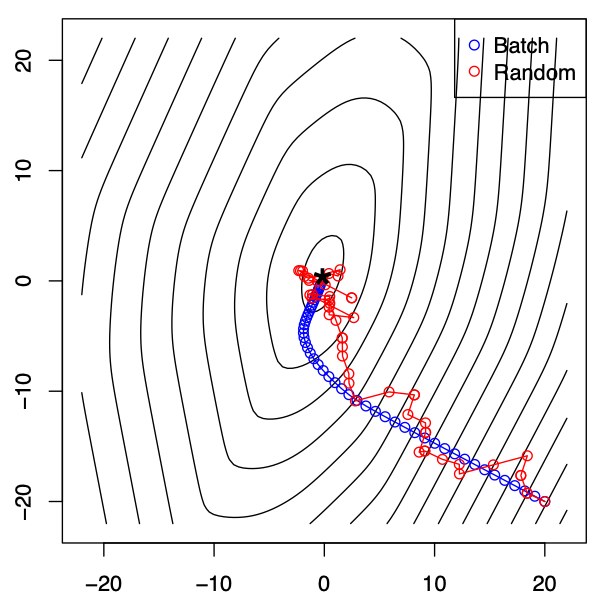
\includegraphics[height=0.6\textheight]{figures/batch-vs-stochastic.png}
    \end{figure}
    \end{column}
    \begin{column}{0.6\textwidth}
        Rule-of-thumb for stochastic methods:
        \begin{itemize}
            \item Stochastic methods work well far from the optimum
            \item But struggles close the the optimum
        \end{itemize}
    \end{column}
    \end{columns}
    (Slides adapted from Ryan Tibshirani)
\end{frame}

\begin{frame}{Minibatch Gradient}
\begin{itemize}
\item What can we say about the minibatch gradient? It's random.
What's its expectation?
%\item What's the expected value of the \textbf{minibatch gradient}?
\begin{eqnarray*}
\ex\left[\del\hat{R}_{N}(w)\right] & = & \frac{1}{N}\sum_{i=1}^{N}\ex\left[\del_{w}\ell(f_{w}(x_{m_{i}}),y_{m_{i}})\right]\\
& = & \ex\left[\del_{w}\ell(f_{w}(x_{m_{1}}),y_{m_{1}})\right]\\
& = & \sum_{i=1}^{n}\pr\left(m_{1}=i\right)\del_{w}\ell(f_{w}(x_{i}),y_{i})\\
& = & \frac{1}{n}\sum_{i=1}^{n}\del_{w}\ell(f_{w}(x_{i}),y_{i})\\
& = & \del\hat{R}_{n}(w)
\end{eqnarray*}
\end{itemize}

%\begin{itemize}
%\item \emph{Technical note:} We only assumed that each point in the minibatch
%is equally likely to be any of the $n$ points in the batch -- no
%independence needed. So still true if we're sampling without replacement.
%Still true if we sample one point randomly and reuse it $N$ times.
%\end{itemize}
\end{frame}
%
\begin{frame}{Minibatch Gradient Properties}
\begin{itemize}
\item Minibatch gradient is an \textbf{unbiased estimator} for the {[}full{]}
batch gradient: 
\[
\ex\left[\del\hat{R}_{N}(w)\right]=\del\hat{R}_{n}(w)
\]
\item The bigger the minibatch, the better the estimate. 
    $$
        \frac{1}{N}\text{Var}\pb{\del\hat{R}_1(w)} = 
        \text{Var}\pb{\del\hat{R}_N(w)}
        $$
\item Tradeoffs of minibatch size:
\begin{itemize}
\item Bigger $N$ $\implies$Better estimate of gradient, but slower (more
data to touch)
\item Smaller $N$ $\implies$Worse estimate of gradient, but can be quite
fast 
\end{itemize}
\end{itemize}
\end{frame}
%
\begin{frame}
    {Convergence of SGD}
    \begin{itemize}
        \item For convergence guarantee, use \textbf{diminishing step sizes},
            e.g. $\eta_k = 1/k$ (dampens noise in step direction)
        \item Theoretically, GD is much faster than SGD in terms of convergence rate  
            \begin{itemize}
                \item much faster to add a digit of accuracy on the minimum
                \item but most of that benefit happens once you're already pretty close
            \end{itemize}
        \item However, in many ML problems we don't care about optimizing to high accuracy
    \end{itemize}
\end{frame}
%
\begin{frame}{Step Sizes in Minibatch Gradient Descent}
\begin{block}{Minibatch Gradient Descent (minibatch size $N$)}
\begin{itemize}
\item initialize $w=0$
\item repeat
\begin{itemize}
\item randomly choose $N$ points $\left\{ (x_{i},y_{i})\right\} _{i=1}^{N}\subset\cd_{n}$
\item $w\gets w-\eta\left[\frac{1}{N}\sum_{i=1}^{N}\del_{w}\ell(f_{w}(x_{i}),y_{i})\right]$
\end{itemize}
\end{itemize}
\end{block}

    \begin{itemize}
        \item For SGD, fixed step size can work well in practice.
        \item Typical approach: Fixed step size reduced by constant factor
whenever validation performance stops improving. 
\item Other tricks: Bottou (2012), ``Stochastic gradient descent tricks''
    \end{itemize}
\end{frame}
%
\begin{frame}{Summary}
\begin{itemize}
\item \textbf{Gradient descent} or \textbf{``full-batch'' gradient descent}
\begin{itemize}
\item Use full data set of size $n$ to determine step direction
\end{itemize}

\item \textbf{Minibatch gradient descent}
\begin{itemize}
\item Use a random subset of size $N$ to determine step direction

%\item Yoshua Bengio says\footnote{See Yoshua Bengio's ``Practical recommendations for gradient-based
%training of deep architectures'' \url{http://arxiv.org/abs/1206.5533}.}:
%\begin{itemize}
%\item $N$ is typically between $1$ and few hundred
%\item $N=32$ is a good default value
%\item With $N\ge10$ we get computational speedup (per datum touched)
%\end{itemize}
\end{itemize}

\item \textbf{Stochastic gradient descent}
\begin{itemize}
\item Minibatch with $N=1$.
\item Use a single randomly chosen point to determine step direction.
\end{itemize}
\end{itemize}

    These days terminology isn't used so consistently, so always clarify
    the {[}mini{]}batch size.

    SGD is much more efficient in time and memory cost and has been quite successful in large-scale ML.
\end{frame}

\section{Practical Comparison of GD vs SGD}
\begin{frame}
    {Logistic regression with $\ell_2$ regularization}
        Batch methods converge faster 
    \begin{figure}
        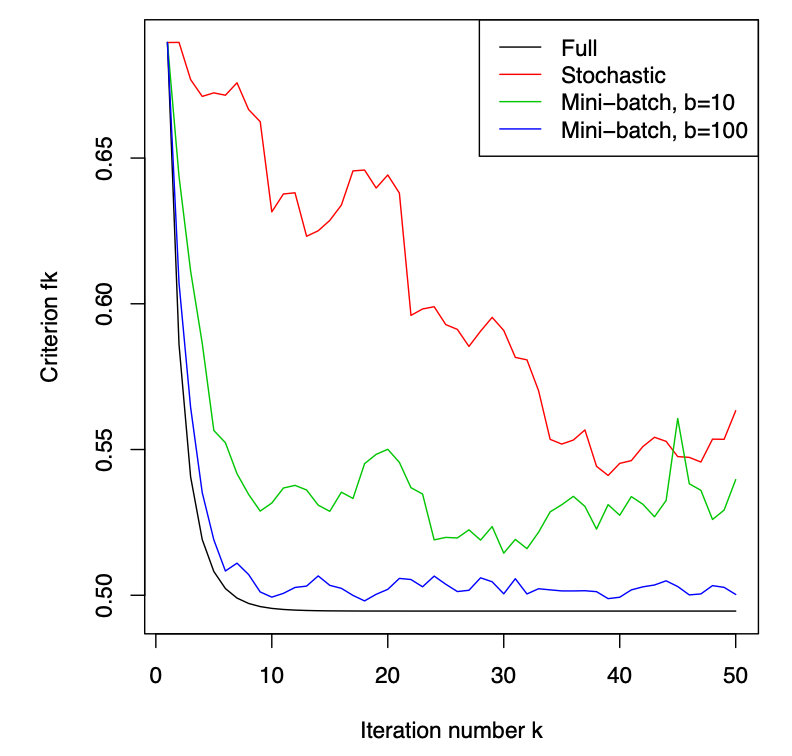
\includegraphics[height=0.7\textheight]{figures/logistic-sgd-loss}
    \end{figure}
    \vspace{-2em}
    (Example from Ryan Tibshirani)
\end{frame}

\begin{frame}
    {Logistic regression with $\ell_2$ regularization}
        Stochastic methods are computationally more efficient 
    \begin{figure}
        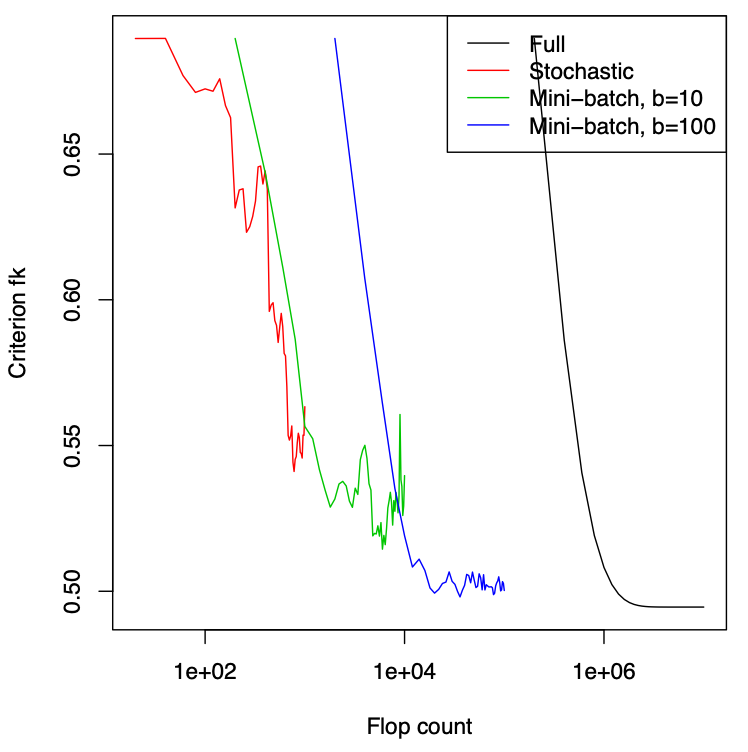
\includegraphics[height=0.7\textheight]{figures/logistic-sgd-flop}
    \end{figure}
    \vspace{-2em}
    (Example from Ryan Tibshirani)
\end{frame}

\begin{frame}
    {Logistic regression with $\ell_2$ regularization}
        Batch methods are much faster close to the optimum 
    \begin{figure}
        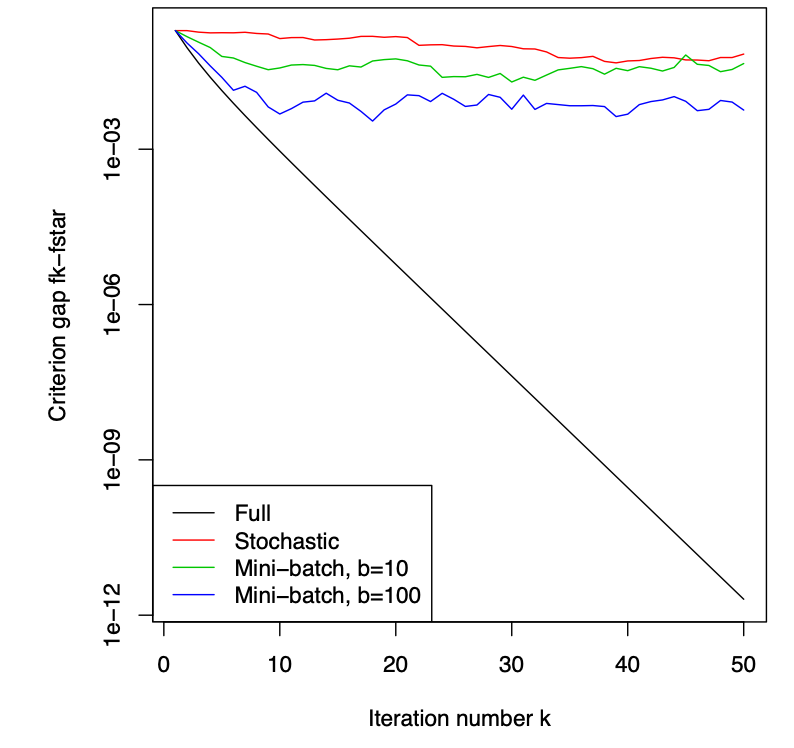
\includegraphics[height=0.7\textheight]{figures/logistic-sgd-optimality}
    \end{figure}
    \vspace{-2em}
    (Example from Ryan Tibshirani)
\end{frame}

\end{document}
